\documentclass[border=8pt]{standalone}
\usepackage{fontspec}
\setmainfont{TeX Gyre Heros}
\setsansfont{TeX Gyre Heros}
\usepackage{tikz}
\usetikzlibrary{arrows.meta,positioning,shapes.geometric,shapes.misc,shapes.symbols,fit,backgrounds,calc,chains}
\definecolor{ink}{HTML}{111827}
\definecolor{band}{HTML}{F3F4F6}
\definecolor{band2}{HTML}{E5E7EB}
\definecolor{accent}{HTML}{1D4ED8}
\definecolor{accentlight}{HTML}{DBEAFE}
\definecolor{warn}{HTML}{B91C1C}
\definecolor{warnlight}{HTML}{FEE2E2}
\definecolor{ok}{HTML}{047857}
\definecolor{oklight}{HTML}{D1FAE5}
\tikzset{
  >={Stealth[length=2.6mm]},
  box/.style={draw=ink, line width=0.6pt, rounded corners=9pt, fill=white, align=center,
              inner sep=4pt, font=\small},
  pill/.style={box, rounded corners=13pt},
  key/.style={box, fill=accentlight, draw=accent, line width=0.9pt},
  soft/.style={box, fill=band},
  dec/.style={draw=ink, line width=0.6pt, diamond, aspect=2.2, align=center, inner sep=1.5pt,
              font=\footnotesize, fill=white},
  arr/.style={->, draw=ink, line width=0.6pt},
  darr/.style={->, draw=ink, line width=0.6pt, dashed},
  lbl/.style={font=\footnotesize, fill=white, inner sep=1.5pt},
  layer/.style={draw=band2, fill=band, rounded corners=6pt},
  title/.style={font=\bfseries\small, align=left, anchor=west},
}
\begin{document}
\sffamily\hyphenpenalty=10000\exhyphenpenalty=10000

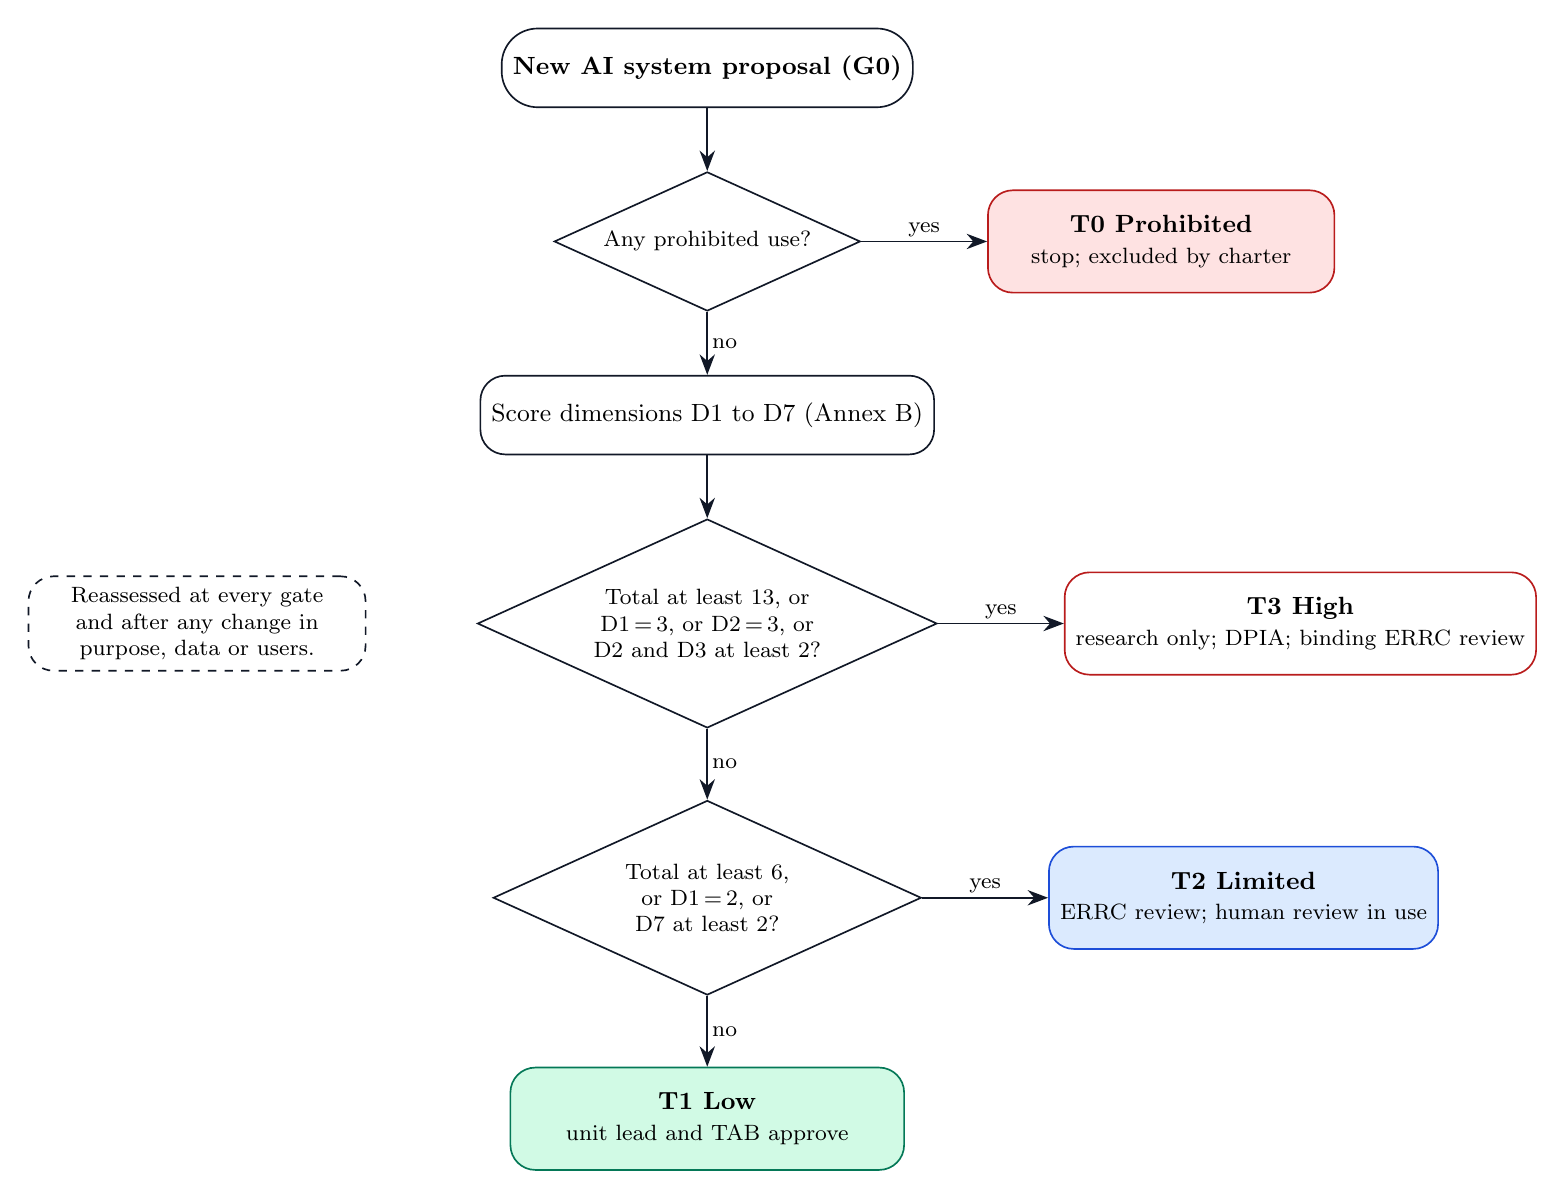
\begin{tikzpicture}[node distance=9mm and 12mm]
\node[pill, minimum width=50mm, minimum height=10mm] (start) {\textbf{New AI system proposal (G0)}};
\node[dec, below=8mm of start, text width=30mm] (p) {Any prohibited use?};
\node[box, draw=warn, fill=warnlight, minimum width=44mm, minimum height=13mm, right=16mm of p] (t0) {\textbf{T0 Prohibited}\\{\footnotesize stop; excluded by charter}};
\node[box, minimum width=50mm, minimum height=10mm, below=8mm of p] (score) {Score dimensions D1 to D7 (Annex B)};
\node[dec, below=8mm of score, text width=36mm] (h) {Total at least 13, or D1\,=\,3, or D2\,=\,3, or D2 and D3 at least 2?};
\node[box, draw=warn, minimum width=44mm, minimum height=13mm, right=16mm of h] (t3) {\textbf{T3 High}\\{\footnotesize research only; DPIA; binding ERRC review}};
\node[dec, below=9mm of h, text width=32mm] (l) {Total at least 6, or D1\,=\,2, or D7 at least 2?};
\node[box, draw=accent, fill=accentlight, minimum width=44mm, minimum height=13mm, right=16mm of l] (t2) {\textbf{T2 Limited}\\{\footnotesize ERRC review; human review in use}};
\node[box, draw=ok, fill=oklight, minimum width=50mm, minimum height=13mm, below=9mm of l] (t1) {\textbf{T1 Low}\\{\footnotesize unit lead and TAB approve}};
\draw[arr] (start) -- (p);
\draw[arr] (p) -- node[lbl, above]{yes} (t0);
\draw[arr] (p) -- node[lbl, right]{no} (score);
\draw[arr] (score) -- (h);
\draw[arr] (h) -- node[lbl, above]{yes} (t3);
\draw[arr] (h) -- node[lbl, right]{no} (l);
\draw[arr] (l) -- node[lbl, above]{yes} (t2);
\draw[arr] (l) -- node[lbl, right]{no} (t1);
\node[box, dashed, text width=40mm, font=\footnotesize, left=14mm of h] (note) {Reassessed at every gate and after any change in purpose, data or users.};
\end{tikzpicture}
\end{document}
